%%%%%%%%%%%%%%%%%%%%%%%%%%%%%%%%%%%%%%%%%%%%%%
\section{Hominins}
%%%%%%%%%%%%%%%%%%%%%%%%%%%%%%%%%%%%%%%%%%%%%%

\begin{frame}
\frametitle{Controversies in human evolution: {\it Ardipithecus ramidus}}
\begin{figure}
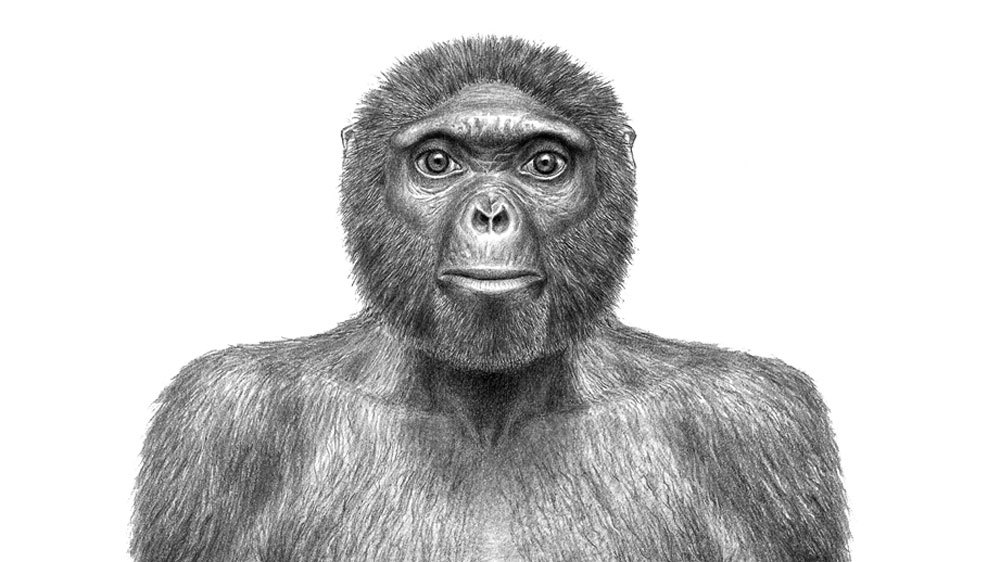
\includegraphics[width=\textwidth]{ardi_crop.jpg}
\end{figure}
`Ardi', 4.4M years old was described as a the oldest fossil relative on the human lineage, a {\it hominin}, and thus more closely related to the human than the chimpanzee. 
\end{frame}

\begin{frame}{Hominin phylogeny inferred using FBD tree prior \& morphological clock.}
\begin{figure}
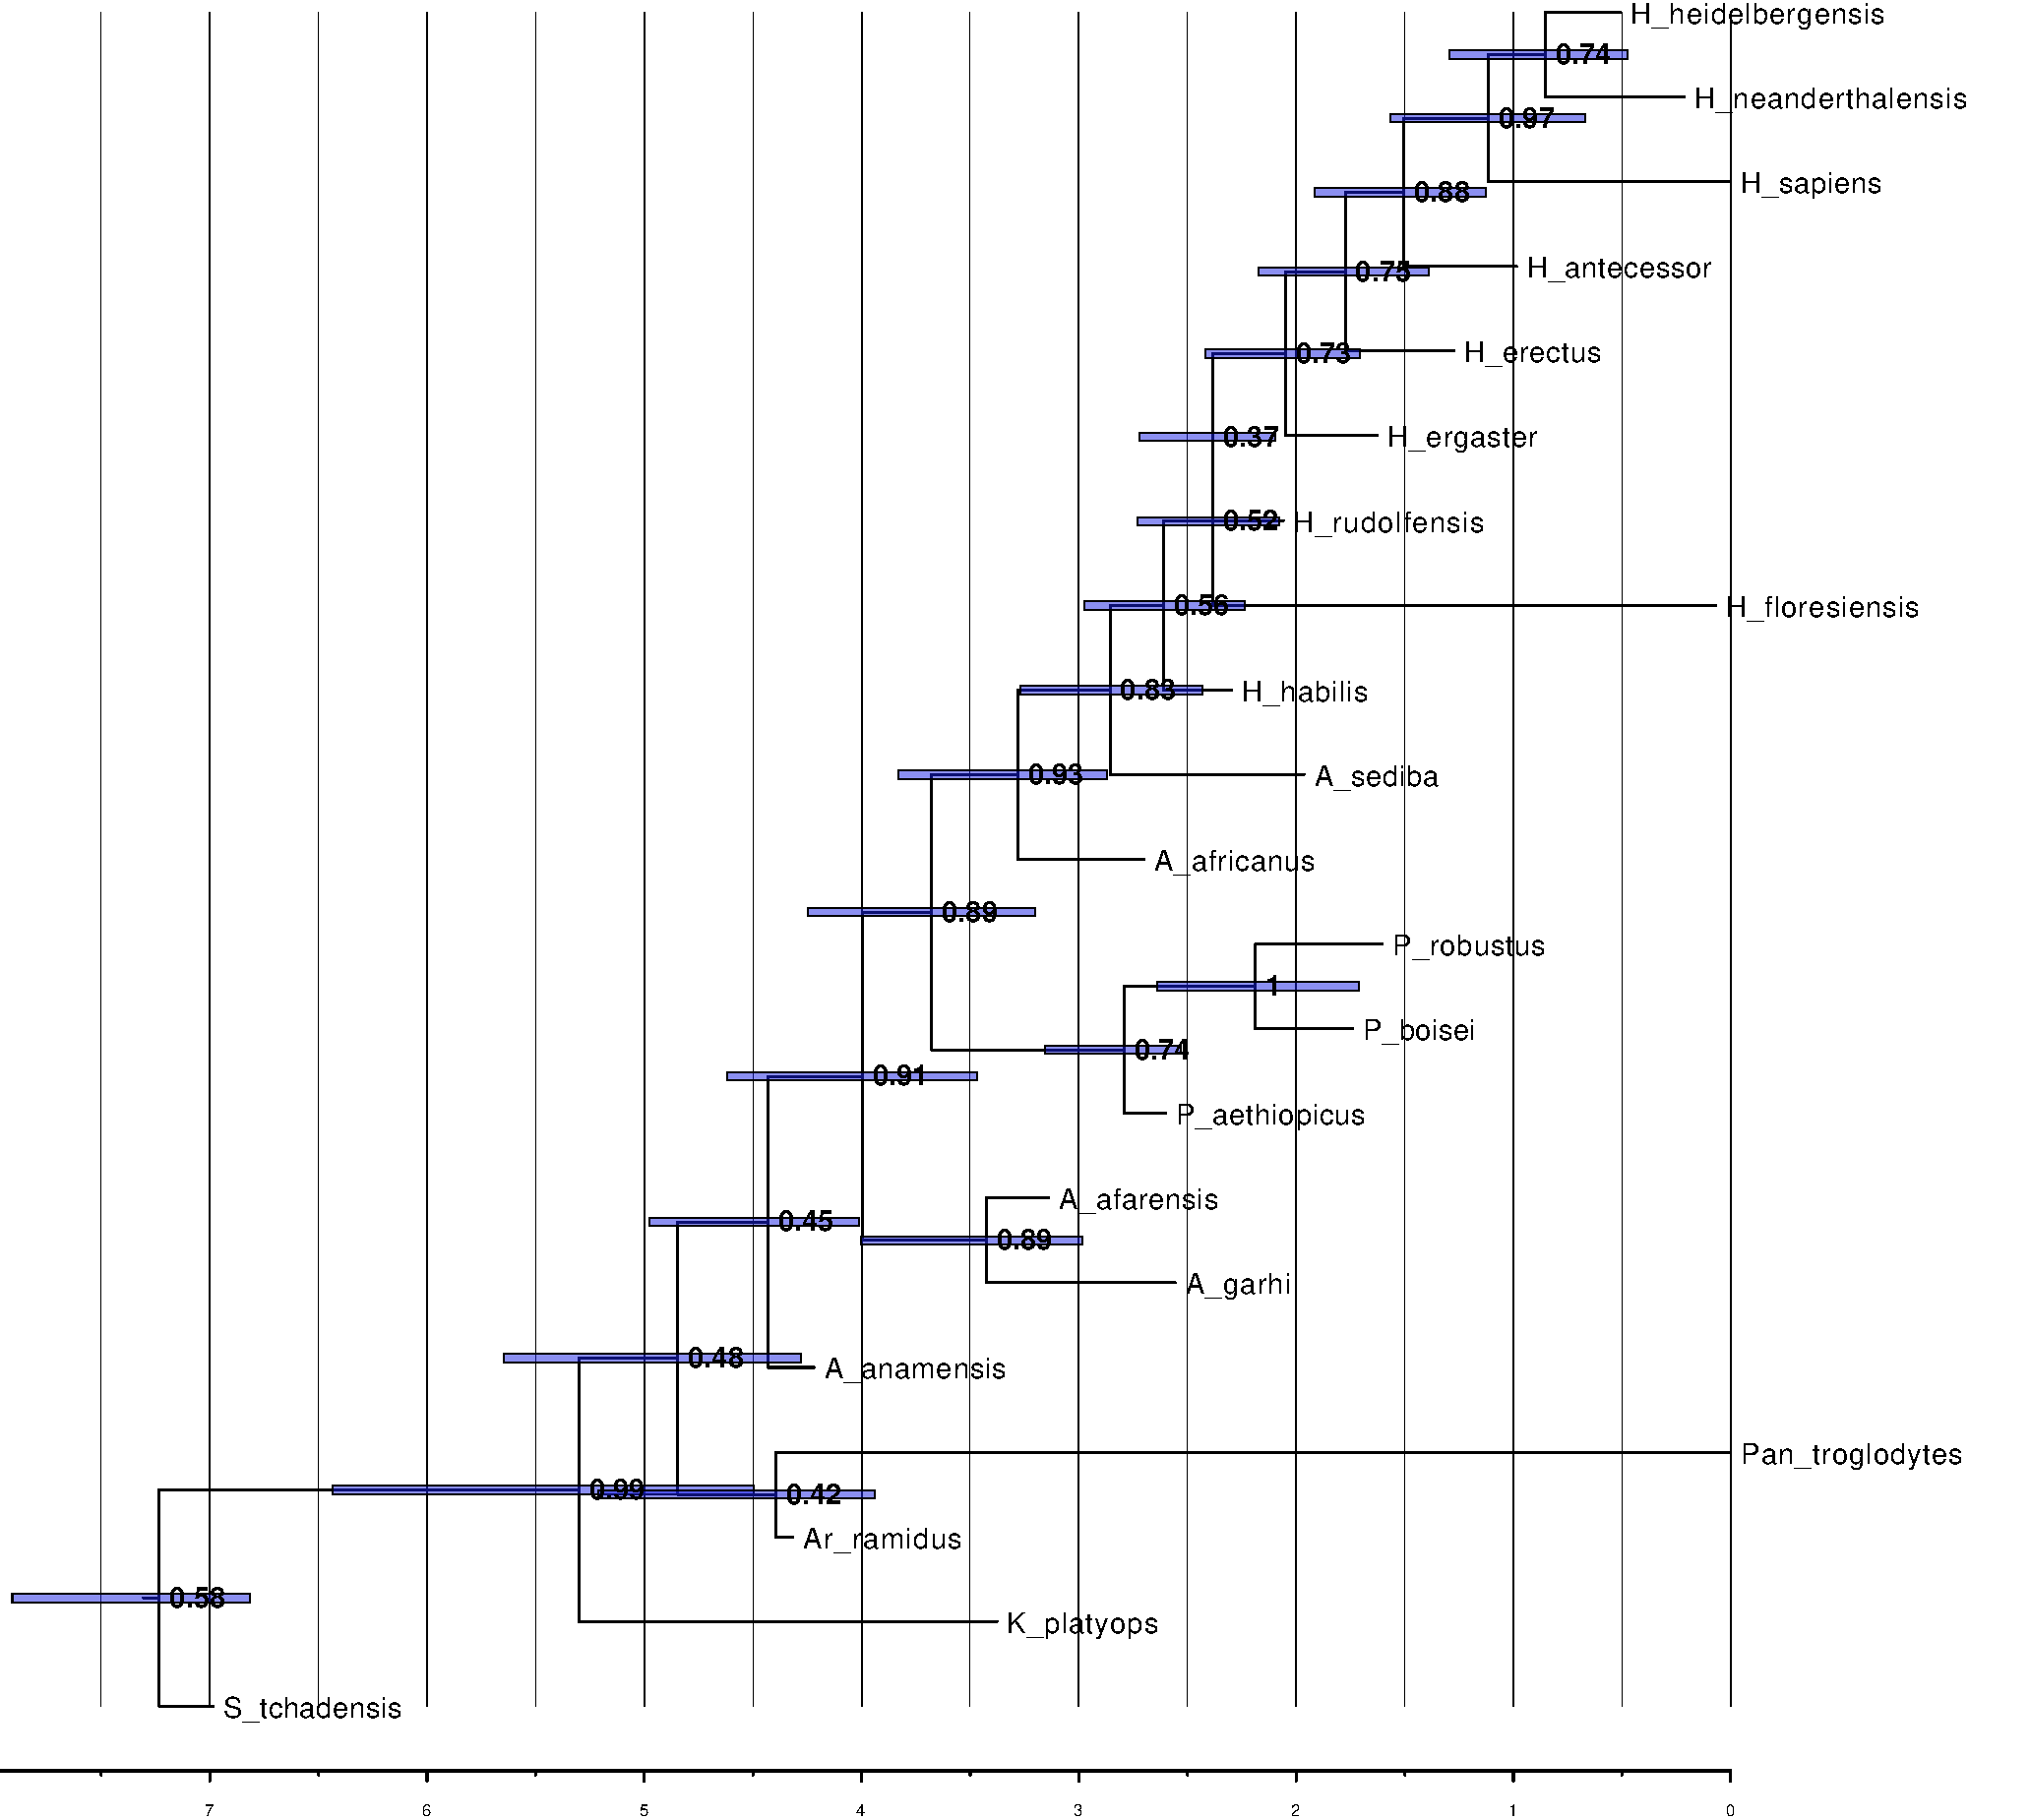
\includegraphics[width=0.75\textwidth]{homininSummaryTree.pdf}
\end{figure}
\end{frame}
